% DRAFT STATUS (2026-09-08): scientific analyses are complete. Resolve the
% author list, ethics/IRB language, code-availability statement, and official
% template/page-limit checks before submission.
%
% Compile this source inside the official ML4H 2026 Overleaf template. The
% official template supplies the conference-specific jmlr.cls.
\documentclass[pmlr,twocolumn,10pt]{jmlr}

\mlhtrack{proceedings}

\newif\iffinal
\finalfalse

\iffinal
  \jmlrvolume{XXX}
  \jmlryear{2026}
  \jmlrworkshop{Machine Learning for Health (ML4H) 2026}
\else
  \jmlrproceedings{}{Submitted to ML4H 2026: \mlhtrackname}
  \jmlrworkshop{Machine Learning for Health (ML4H) 2026}
\fi

\urlstyle{same}
\usepackage{booktabs}
\usepackage{graphicx}
\usepackage[switch]{lineno}

\title[Longitudinal Time in Text-Serialized EHRs]{Do Text-Serialized EHR Models Use Longitudinal Time?\\
Controlled History and Timestamp Stress Tests on EHRSHOT}

\author{Anonymous Author(s)}

\linenumbers

\begin{document}
\maketitle

\begin{center}
\fbox{\parbox{0.92\linewidth}{\textbf{Scientific draft complete.}
The frozen one-time held-out analysis is final. Resolve authorship, ethics/IRB,
code availability, and official template checks before submission.}}
\end{center}

\begin{abstract}
Longitudinal electronic health records (EHRs) contain both clinical events and
irregular temporal structure, yet adding timestamps to text-serialized EHRs has
not consistently improved prediction. Existing comparisons can conflate the
value of earlier history, elapsed time, event--time correspondence, and the
clinical evidence displaced by temporal tokens. We introduce a controlled,
patient-balanced evaluation on four EHRSHOT task families. Using identical
strictly pre-prediction events, we compare chronological order without elapsed
time, correct prediction-relative time, reversed earlier gaps, and shuffled
earlier time labels; the most recent window remains correct under every temporal
falsification. Our primary interface embeds the flat 8,192-token history with
frozen Qwen3-Embedding-0.6B and fits task-specific logistic readouts. In a
one-time held-out evaluation of 4,343 patient--task instances, correct-time
history achieved equal-weight macro-AUROC 0.646. It did not outperform the
latest-window baseline (difference $-0.014$, 95\% paired-bootstrap CI $-0.032$
to $0.003$; Holm-adjusted $p=0.224$) or the mean prediction from three
shuffled-time conditions (difference $0.002$, 95\% CI $-0.001$ to $0.006$;
Holm-adjusted $p=0.224$). A code-count baseline reached macro-AUROC 0.711.
Correct time modestly improved over order alone for anemia, but this effect did
not generalize across tasks. These results indicate that textual timestamps do
not reliably add linearly accessible predictive signal to this frozen flat
embedding, despite strong task-specific discrimination for anemia.
\end{abstract}

\begin{keywords}
electronic health records, temporal representation, foundation models,
clinical prediction, robustness evaluation
\end{keywords}

\paragraph*{Data and Code Availability}
EHRSHOT is available to approved researchers under a data use agreement and
cannot be redistributed by the authors \citep{wornow2023ehrshot}. Patient-level
cohorts, serialized histories, summaries, embeddings, labels, and predictions
remain in governed storage. An anonymized implementation is planned as review
supplemental material; this statement must be changed before submission if that
supplement is not provided.

\paragraph*{Institutional Review Board (IRB)}
This study is a secondary analysis of de-identified EHRSHOT data under its data
use agreement. \textbf{[REQUIRED BEFORE SUBMISSION: insert the applicable IRB
approval, exemption, Not Human Subjects Research determination, or an
institutionally supported explanation of non-applicability. If allowed for
anonymous review, state that identifying approval information will be provided
upon acceptance.]}

\section{Introduction}
\label{sec:introduction}

Structured EHRs represent clinical trajectories as irregular sequences of
diagnoses, procedures, medications, and measurements. Their timing can convey
disease progression, monitoring intensity, and transitions in care, but long
records also contain recurrence, missingness, and copy-forwarded information.
Recent long-context EHR models benefit from additional history on many tasks,
while remaining sensitive to repetition and irregular observation
\citep{wornow2025context}. Models trained with explicit temporal components can
also benefit from time encodings \citep{pang2021cehrbert}. Controlled studies of
temporal tokenization nevertheless report task- and distribution-dependent
effects rather than one uniformly superior encoding
\citep{alattrach2025tokenization,liu2025temporal}. These findings do not
establish whether a frozen text embedding uses the correct assignment of
elapsed time to clinical events.

General-purpose embedding models offer an appealing alternative to EHR-specific
pretraining because structured codes can be serialized as text. Hegselmann
et~al. showed that Qwen3-Embedding-8B with logistic-regression readouts can be
competitive across EHRSHOT, but their default serialization retained the most
recent occurrence of each code and simple timestamp additions did not improve
the aggregate result \citep{hegselmann2026llm}. This leaves an ambiguity: time
might be unhelpful, the model might not use its textual representation, or
preprocessing and finite context might remove the recurrence and alignment
signals needed to observe an effect.

We address this ambiguity with content-matched temporal stress tests. The work
does not propose a new foundation model or claim causal or clinical utility.
Instead, it separates four questions: whether earlier history improves on the
latest observation window; whether explicit elapsed time improves on event
order; whether correct event--time correspondence matters; and whether these
signals behave differently under flat embedding, one-pass summarization, and
window-level sequence aggregation. Our contributions are:

\begin{enumerate}
  \item a leakage-controlled, MEDS-native, patient-balanced evaluation spanning
  four EHRSHOT task families;
  \item temporal falsifications that change label indices without rearranging
  clinical events, preserving the final window and content matching;
  \item a complete direct-embedding evaluation, secondary validation of a
  window-sequence model, and fail-closed documentation of an incomplete
  summary interface; and
  \item paired patient-level uncertainty estimates plus audits of fidelity,
  truncation, recurrence, and perturbation strength.
\end{enumerate}

\section{Related Work}
\label{sec:related}

EHRSHOT provides de-identified longitudinal records for 6,739 patients, 15
prediction tasks in four clinical families, and canonical patient splits
\citep{wornow2023ehrshot}. We use its structured event data through the Medical
Event Data Standard (MEDS), which is designed to improve portability and
reproducibility in health-AI workflows \citep{mcdermott2026meds}. Our study is a
derived patient-balanced evaluation rather than an official all-label EHRSHOT
leaderboard submission.

Qwen3 Embedding offers instruction-aware models at 0.6B, 4B, and 8B scales
\citep{zhang2025qwen3embedding}. The 0.6B model makes the complete controlled
matrix computationally feasible; a prespecified runtime-only gate admits a
subset of 8B M1 confirmations without using outcomes to select cells. The
one-pass compression approach is motivated by abstraction as a long-context
interface, but it is neither recursive nor a retrieval system and should not be
described as a RAPTOR implementation \citep{sarthi2024raptor}. PaReGTA instead
combines visit-level templated text, contrastively adapted sentence embeddings,
and temporal pooling, illustrating that explicit temporal structure may be more
useful when it is learned and aggregated rather than appended to one flat text
\citep{yoon2026paregta}.

This work evaluates prediction from an observed history. It does not estimate
the causal effect of changing when an intervention occurs; methods such as
Earliest Disagreement Q-Evaluation address that distinct irregular-time policy
evaluation problem under causal assumptions \citep{wald2025time}.

\section{Methods}
\label{sec:methods}

\subsection{Study design and prediction tasks}

The unit of analysis is one selected patient--task--prediction-time instance.
The four tasks were locked before the engineering pilot's embedding performance
was examined: (1) whether the next qualifying hemoglobin result is abnormal
(\texttt{lab\_anemia}); (2) readmission within 30 days
(\texttt{guo\_readmission}); (3) a first hypertension diagnosis within one year
(\texttt{new\_hypertension}); and (4) a chest-radiograph finding rather than
``No Finding'' (\texttt{chexpert}). We use each task's official prediction time
$T$ and preserve the official patient-level train, validation, and held-out
split assignments. Development and model selection use train and validation
only; the held-out split remains inaccessible until a cryptographically hashed
analysis manifest is frozen.

\begin{table*}[t]
\floatconts
  {tab:cohort}
  {\caption{Locked patient-balanced cohort. Test counts were accessed only by
  the frozen one-time evaluation.}}
  {\begin{tabular}{lrrrrrr}
  \toprule
  Task & Train & Train $\%+$ & Validation & Val. $\%+$ & Test & Test $\%+$ \\
  \midrule
  Anemia & 2,092 & 47.3 & 1,991 & 45.8 & 2,002 & 46.4 \\
  Readmission & 1,337 & 5.8 & 1,191 & 5.4 & 1,190 & 5.3 \\
  New hypertension & 792 & 14.5 & 781 & 15.4 & 755 & 15.9 \\
  CheXpert & 250 & 64.4 & 395 & 66.6 & 396 & 67.4 \\
  \midrule
  Total & 4,471 & --- & 4,358 & --- & 4,343 & --- \\
  \bottomrule
  \end{tabular}}
\end{table*}

For each patient, duplicate official prediction-time groups are excluded before
ranking, regardless of whether their labels agree. Remaining official times are
sorted and one is chosen by the minimum SHA-256 rank over dataset release,
task, split, patient, frozen seed, and sorted eligible prediction-time index.
The rule does not use outcome, event history, record length, row order, or model
performance. This produces 8,829 train/validation instances (Table
\ref{tab:cohort}).

\subsection{Leakage control, deduplication, and windows}

Only events with event time strictly earlier than $T$ are retained. We remove
only exact duplicates over subject, event time, code, numeric value, text value,
unit, and source table, preserving recurrence whenever any field or timestamp
differs. Prediction-relative half-open windows are
$[T-(i+1)w,T-iw)$, with $w=30$ days for laboratory, imaging, and operational
tasks and $w=90$ days for incident diagnosis. The implementation separately
audits that anemia predicts the next hemoglobin result rather than an incident
diagnosis, readmission inputs exclude the future admission, hypertension follows
the official one-year incident definition, and CheXpert prediction precedes the
report or finding.

\subsection{Controlled representations}

The complete-history stress test holds retained events and their chronological
order fixed. C0 includes order but no elapsed-time labels. C1 attaches correct,
compact, prediction-relative window labels. C2 assigns the observed earlier gap
multiset in reverse order while preserving chronology, total span, and the
correct final window. C3 shuffles earlier time-label indices using seeds
20260815, 20260816, and 20260817 while retaining the correct final window.
Clinical event arrays are never rearranged by C2 or C3. Histories without an
effective perturbation are excluded from the applicable perturbable-subset
contrast rather than assigned a fictitious change.

Four baselines reduce or remove information: B1 retains only the latest
nonempty window; B2 retains the latest occurrence of each code across history,
approximating the closest predecessor's reduction; B3 is a log-transformed code
count with penalized logistic regression; and B4 predicts training prevalence.
B1 and B2 are separate baselines, not temporal conditions.

\subsection{Modeling approaches}

\paragraph{M1: direct serialization.}
The flat serialized document is truncated to 8,192 tokens and embedded by a
frozen Qwen3-Embedding-0.6B model. Finite vectors are promoted to FP32 and
explicitly L2-normalized before immutable caching. For each task and
representation, a penalized logistic regression is selected from
$C\in\{0.01,0.1,1,10\}$ by validation AUROC, choosing the smallest $C$ under an
exact tie. A separate throughput benchmark, blind to outcome performance,
selected a feasible prefix of prespecified Qwen3-Embedding-8B confirmations in
the order C1, C3, B1, and B2. Consequently, 8B results are secondary
scale-sensitivity analyses and do not form a complete four-task matrix.

\paragraph{M2: one-pass summary embedding.}
M2 was designed to compress the same content-matched source evidence with an
on-premise \texttt{nvidia/Qwen3.6-35B-A3B-NVFP4} endpoint before applying the
M1 embedding and logistic readout. Versioned attempts used deterministic
decoding and increasingly bounded, structured prompts with exact retention and
contradiction checks. The interface did not complete the prespecified fidelity
and runtime gates within the study period, so it was declared incomplete future
work before held-out access. Partial M2 caches are not analyzed, and M2 never
accessed held-out outcomes.

\paragraph{M3: per-window sequence aggregation.}
Each of at most 64 recent nonempty windows is independently embedded with the
frozen 0.6B model using 512 tokens per window. A fixed seed-20260819 projection
maps embeddings to 256 dimensions. The primary sequence head is a one-layer,
128-hidden-unit, unidirectional gated recurrent unit (GRU)
\citep{cho2014gru} with input dropout 0.1, trained with AdamW
\citep{loshchilov2019adamw}
(learning rate $10^{-3}$, weight decay 0.01, batch size 32) for at most 50
epochs. Early stopping uses validation AUROC with patience 5 and validation log
loss only to resolve AUROC ties. Training is repeated under seeds 20260815--17.
Mean pooling followed by logistic regression is the capacity comparator.
The completed validation reference yielded macro-AUROC 0.622, below M1's
0.694; therefore M3 remained a secondary validation-only analysis and did not
access held-out outcomes.

\subsection{Evaluation and approach selection}

We report per-task and equal-weight four-task macro-AUROC, AUPRC, Brier score,
log loss, and calibration slope/intercept where identifiable. Paired contrasts
resample patients within task for 2,000 bootstrap replicates and then weight the
four task estimates equally. Prespecified contrasts are C1--C0, C1--C2,
C1--each C3 seed, C1--B1, and C1--B2, for both complete-cohort and eligible
perturbable subsets as applicable. We also report C3 seed variability, retained
history, recurrence, truncation, perturbation strength, runtime, peak memory,
and storage. Holm correction controls the family-wise error rate for the two
co-primary panel contrasts \citep{holm1979multiple}; Benjamini--Hochberg controls
the false discovery rate across the prespecified per-task secondary family
\citep{benjamini1995fdr}.

The original selection rule compared complete-correct C1 validation results and
required a challenger to improve equal-weight macro-AUROC by at least 0.005;
otherwise the simplicity order M1, M2, then M3 applied. M1 completed every
required baseline and falsification. M3 completed its validation reference but
underperformed M1 (0.622 versus 0.694 macro-AUROC), while M2 did not pass its
fidelity/runtime gates. The scope was therefore frozen to M1 as the sole
held-out interface, with M3 retained as secondary validation evidence and M2 as
incomplete future work. This decision and all M1 settings were hash-pinned
before the one-time held-out evaluation and were not revised afterward.

\section{Results}
\label{sec:results}

\subsection{Cohort, integrity, and frozen scope}

The final foundation selected 4,471 training, 4,358 validation, and 4,343
held-out instances across four tasks. Content matching passed, C2/C3 altered
label indices rather than clinical arrays, and the patient-window metadata
mirrored every embedding row. After validation, M1 was frozen as the primary
interface; M3 remained secondary validation evidence, and M2 was designated
incomplete future work. The held-out split was then evaluated once under the
frozen manifest, with no post-access protocol modification.

\subsection{Development evidence}

Correct relative time yielded M1 validation macro-AUROC 0.694 compared with
0.690 for order alone. The paired difference was 0.0033 (95\% CI, $-0.0019$ to
$0.0085$). M3's C1 validation macro-AUROC was 0.622, so it did not displace M1.

\begin{table}[t]
\floatconts
  {tab:m1validation}
  {\caption{Completed Qwen3-Embedding-0.6B M1 validation AUROC. Macro values
  weight tasks equally. C2 and C3 macro values use eligible perturbable subsets
  and are therefore not direct complete-cohort columns.}}
  {\begin{tabular}{lrrrrr}
  \toprule
  Task & C0 & C1 & B1 & B2 & B3 \\
  \midrule
  Anemia & .813 & .823 & .820 & .789 & .828 \\
  Readmission & .713 & .712 & .715 & .632 & .673 \\
  New hypertension & .696 & .693 & .680 & .734 & .724 \\
  CheXpert & .541 & .546 & .568 & .555 & .584 \\
  \midrule
  Equal-weight macro & .690 & .694 & .696 & .678 & .702 \\
  \bottomrule
  \end{tabular}}
\end{table}

\subsection{One-time held-out M1 evaluation}

\begin{figure}[t]
  \centering
  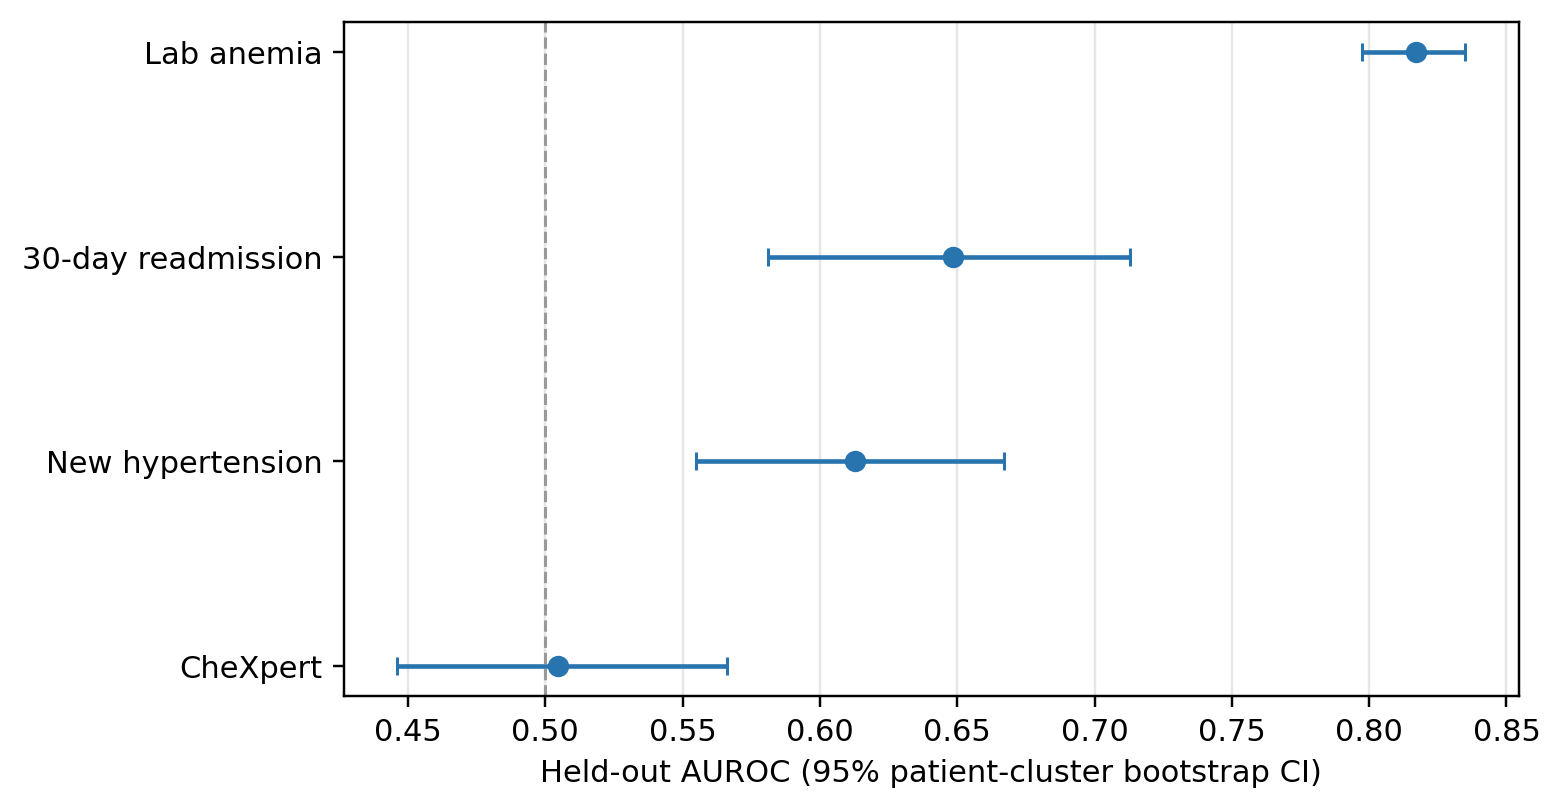
\includegraphics[width=\linewidth]{figures/figure_main_performance.png}
  \caption{Held-out discrimination of the frozen M1 conditions and baselines.
  Panel macro values weight the four tasks equally.}
  \label{fig:mainperformance}
\end{figure}

Table~\ref{tab:test} shows task-level C1 performance. The equal-weight panel
macro-AUROC was 0.646 (95\% CI, 0.618--0.672), with macro-AUPRC 0.442, Brier
score 0.146, and log loss 0.452. Discrimination varied substantially: anemia
AUROC was 0.817, whereas CheXpert AUROC was 0.505. CheXpert AUPRC was 0.695 in
the setting of 67.4\% outcome prevalence and should not be read as evidence of
ranking discrimination.

\begin{table}[t]
\floatconts
  {tab:test}
  {\caption{Frozen M1 C1 one-time held-out performance.}}
  {\begin{tabular}{lrrrr}
  \toprule
  Task & $n$ & AUROC & AUPRC & Brier \\
  \midrule
  Anemia & 2,002 & .817 & .768 & .174 \\
  Readmission & 1,190 & .649 & .085 & .050 \\
  New hypertension & 755 & .613 & .222 & .131 \\
  CheXpert & 396 & .505 & .695 & .229 \\
  \midrule
  Equal-weight macro & 4,343 & .646 & .442 & .146 \\
  \bottomrule
  \end{tabular}}
\end{table}

\begin{figure}[t]
  \centering
  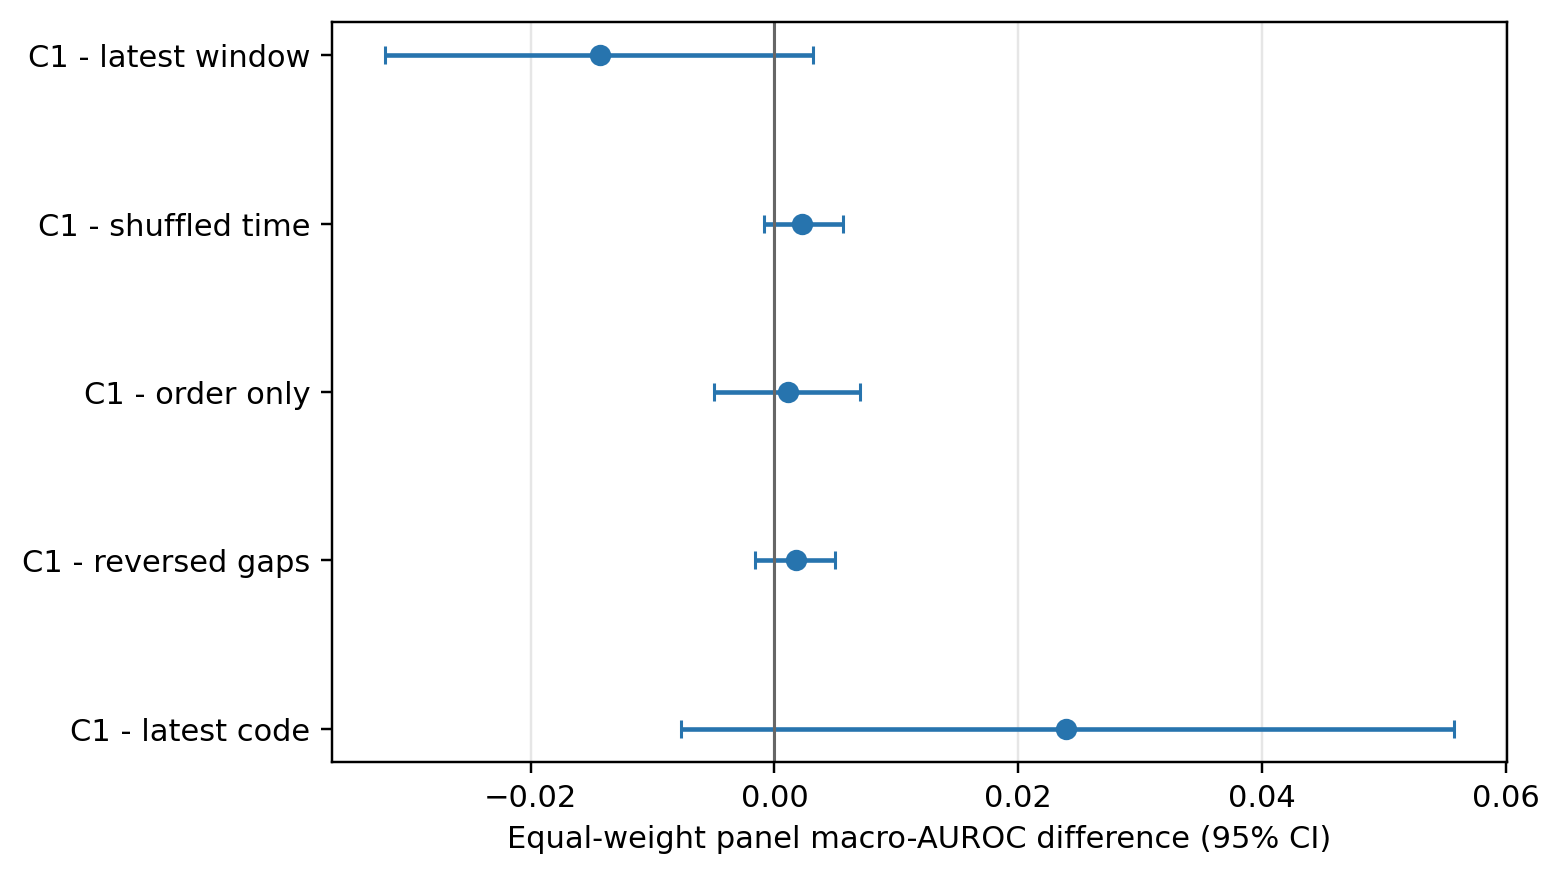
\includegraphics[width=\linewidth]{figures/figure_primary_contrasts.png}
  \caption{Paired patient-cluster bootstrap contrasts for the frozen held-out
  analysis. Intervals crossing zero indicate no detectable difference.}
  \label{fig:contrasts}
\end{figure}

Correct timing did not outperform the latest-window baseline: C1--B1 was
$-0.014$ (95\% CI, $-0.032$ to 0.003; Holm-adjusted $p=0.224$). Nor did it
outperform the mean prediction across three shuffled-time seeds: C1--C3 was
0.002 (95\% CI, $-0.001$ to 0.006; Holm-adjusted $p=0.224$). C1--C0 was 0.001
(95\% CI, $-0.005$ to 0.007), and C1--C2 was 0.002 (95\% CI, $-0.002$ to
0.005) on the perturbable subset. The code-count baseline achieved the highest
macro-AUROC (0.711), exceeding C1 by 0.066. At task level, anemia was the only
task with a detectable C1--C0 effect (0.009; 95\% CI, 0.003--0.015; BH-adjusted
$q=0.012$); the effect did not generalize across the other tasks.

\section{Discussion}
\label{sec:discussion}

In this frozen four-task evaluation, a flat frozen embedding with a linear
readout did not show a reliable aggregate benefit from correct textual time
labels. The co-primary comparisons against latest-window history and shuffled
earlier labels were null, and order-only and reversed-gap conditions were also
similar. The strongest conventional comparator was the code-count model. These
results caution against assuming that a long-context text encoder uses explicit
timestamps merely because they are present in the input.

The positive anemia-specific C1--C0 contrast suggests that temporal labels may
still matter for selected outcomes. Its absence in the panel-level result and
the other three tasks argues for heterogeneity rather than a universal claim
that dates never help. M3 did not improve on M1 in validation, so added
sequential capacity alone did not rescue performance in this implementation.
M2 remains a useful future direction, but its incomplete fidelity/runtime gate
precludes any empirical claim here.

The study has important limitations. It uses four selected EHRSHOT tasks and a
derived patient-balanced cohort rather than all labels in the official
leaderboard. EHRSHOT is a de-identified, single-system dataset, and its recorded
timing reflects both physiology and healthcare observation. Windows are not
true encounters because the event table lacks a reliable encounter container.
M1 uses the 0.6B encoder for the complete matrix; runtime-feasible 8B cells are
secondary and cannot provide a four-task 8B macro estimate. M2 was not
completed and therefore cannot support a comparison. We did not perform
external validation, subgroup fairness analysis, or prospective evaluation.
Finally, predictive performance and stress-test sensitivity do not establish
causal understanding, clinical usefulness, or safety.

\section{Conclusion}
\label{sec:conclusion}

We present a controlled framework for separating history coverage, elapsed
time, and event--time alignment in text-serialized longitudinal EHR prediction.
In the frozen one-time held-out evaluation, correct prediction-relative labels
did not improve panel-level performance over the latest window, order alone, or
shuffled earlier labels, and a code-count baseline performed best. A modest
anemia-specific effect supports task-dependent follow-up, while the aggregate
findings argue for falsification controls before attributing predictive gains to
textual representations of longitudinal time.

\bibliography{references}

\appendix

\section{Prespecified reporting checklist}

The camera-ready analysis must identify the dataset and transformation versions,
selection and censoring rules, task-specific windows, all C3 seeds, model and
tokenizer hashes, summary prompt and decoding controls, hyperparameter grids,
approach-selection rule, bootstrap unit and replicate count, truncation and
perturbation audits, runtime and memory, code availability, and the applicable
ethics determination. All test results must originate from one frozen-manifest
execution, and no post-test design change is permitted.

\end{document}
